\section{Concrete Form of the Condition Matrices}
In this section the construction of the condition matrices $\uuline{M}_n$ from
equation \ref{eq:statevector} is considered in more detail.
With the general wave solution equation \ref{eq:gendisplacement} the strain
in layer $n$ tensor evaluates to
\begin{align}
    \epsilon_{ij} = \frac{i}{2} \left(
    (\uline{\vu{e}}_i\cdot \uline{u}(\underline{x}, t))\
    (\uline{\vu{e}}_j\cdot \uline{k}^t_{n})
    + (\uline{\vu{e}}_j\cdot  \uline{u}(\underline{x}, t))\
    (\uline{\vu{e}}_i\cdot \uline{k}^t_{n}) \right) \\ 
    = \frac{i}{2}\sum\limits_{p\in\{L,TH,TV\}} 
    t_p\ \epsilon^t_{ij,p} e^{i(\uline{k}_{p}^t\uline{x} - \omega t)} 
    + r_p\ \epsilon^r_{ij,p}\ e^{i(\uline{k}_{p}^r\uline{x} - \omega t)} \nonumber
\end{align}
with 
\begin{equation}
    \epsilon^t_{ij,p} = \frac{i}{2} \left(
    (\uline{\vu{e}}_i\cdot \uline{p}_p^t) \
    (\uline{\vu{e}}_j\cdot \uline{k}^t_{p})
    + (\uline{\vu{e}}_j\cdot \uline{p}_p^t)\
    (\uline{\vu{e}}_i\cdot \uline{k}^t_{p}) \right)
\end{equation}
and analogously for $\epsilon^r_{ij,p}$. The condition matrix is then constructed
as 
\begin{equation}
    \uuline{M}=\begin{pmatrix}
        |  &  | &  | &  | &  |  &  | \\
    \uline{p}_L^t &  \uline{p}_{TH}^t &  \uline{p}_{TV}^t &
    \uline{p}_L^r &  \uline{p}_{TH}^r &  \uline{p}_{TV}^r  \\
        |  &  | &  | &  | &  |  &  | \\
        C_{55}\epsilon^t_{13,L} & C_{55}\epsilon^t_{13,TH} & 
        C_{55}\epsilon^t_{13,TV} & 
        C_{55}\epsilon^r_{13,L} & C_{55}\epsilon^r_{13,TH} & 
        C_{55}\epsilon^r_{13,TV} \\
        C_{44}\epsilon^t_{23,L} & C_{44}\epsilon^t_{23,TH} & 
        C_{44}\epsilon^t_{23,TV} &
        C_{44}\epsilon^r_{23,L} & C_{44}\epsilon^r_{23,TH} & 
        C_{44}\epsilon^r_{23,TV} \\
        C_{3i}\epsilon^t_{ii,L} & C_{3i}\epsilon^t_{ii,TH} & 
        C_{3i}\epsilon^t_{ii,TV} &
        C_{3i}\epsilon^r_{ii,L} & C_{3i}\epsilon^r_{ii,TH} & 
        C_{3i}\epsilon^r_{ii,TV} \\
    \end{pmatrix}
\end{equation}
with Einstein convention implied in the last row, in order to fulfill equation
\ref{eq:statevector}.


\section{Detailed Plots Picturing Scopes of Numerical Instabilites}
The following plots show the reflector from section \ref{sec:reflector} 
calculated with \ttt{TransferMethod()} in comparison to the plots from above with 
\ttt{singleLSEMethod()}.

\begin{figure}[p]
    \centering
    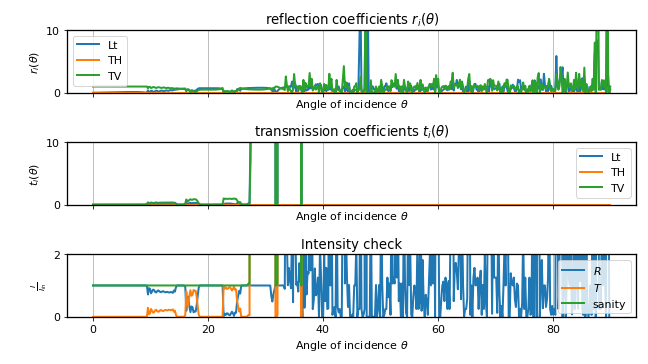
\includegraphics[width=\textwidth]{Example2/TV_at477GHz_transfer.png}
    \caption{Angular Plot with frequency $f=477\si{GHz}$ for TV mode with \ttt{TransferMethod()}}
    \label{fig:anTMM_TV}
\end{figure}
\begin{figure}[p]
    \centering
    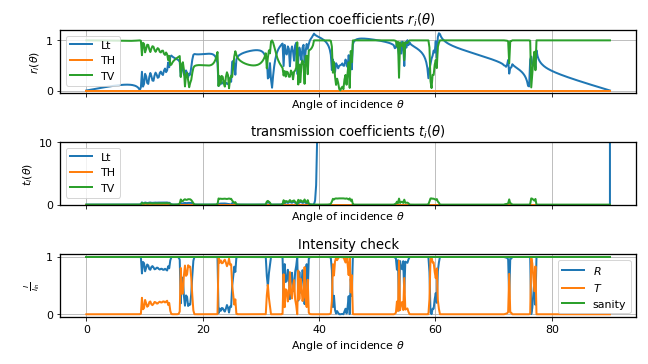
\includegraphics[width=\textwidth]{Example2/TV_at477GHz_singlelse.png}
    \caption{Angular Plot with frequency $f=477\si{GHz}$ for TV mode with \ttt{singleLSEMethod()}}
    \label{fig:anLSE_TV}
\end{figure}

\begin{figure}[p]
    \centering
    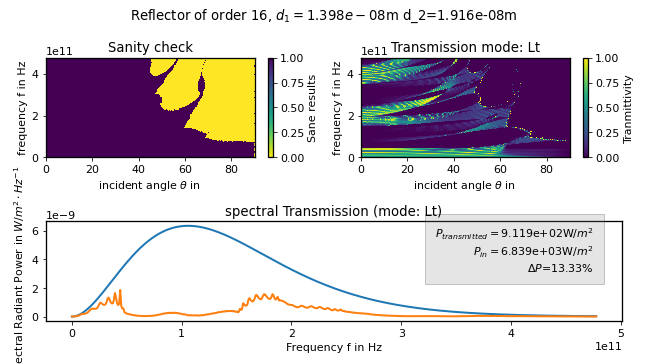
\includegraphics[width=\textwidth]{Example2/L_transfer.png}
    \caption{Overview for \ttt{TransferMethod()} and mode L}
    \label{fig:ovTMM_L}
\end{figure}
\begin{figure}[p]
    \centering
    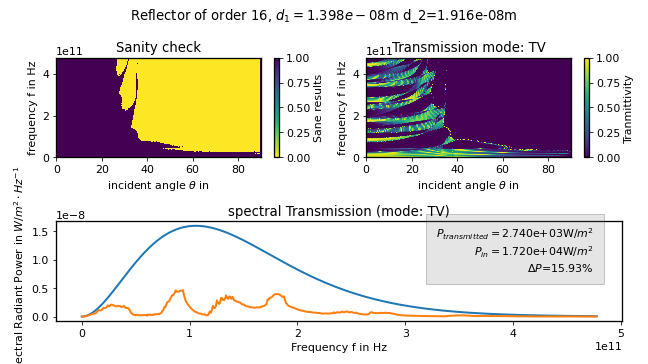
\includegraphics[width=\textwidth]{Example2/TV_transfer.png}
    \caption{Overview for \ttt{TransferMethod()} and mode TV}
    \label{fig:ovTMM_TV}
\end{figure}
 
\newpage
\section{Materials in \ttt{materials.py} }


\begin{table}[h]
    \centering
    \begin{tabular}{c|c|c|c|c|c}
        material & density $\rho$ in $\si{\frac{kg}{m^3}}$   & $c_L$ in $\si{\frac{m}{s}}$  
        &   $c_T$ in $\si{\frac{m}{s}}$   &   $Z_L$ in $10^7\si{\frac{Pa\ s}{m}}$     &   	$Z_T$  in $10^7\si{\frac{Pa\ s}{m}}$ \\ \hline
    GaAs \cite{matprop}
    &       $5317$        &       $4732$        &
        $2485$        &       $2.516 $     &       $1.322 $ \\
    Si \cite{matprop}
      &       $2329$        &       $8476 $        &
        $4725$        &       $1.974 $     &       $1.100 $ \\
    $\si{Si_{0.7}Ge_{0.3}} $\cite{matprop}    &       $3332$        &       $6814$
            &       $3785$        &       $2.271 $     &       $1.261 $ \\
    $\si{AlGaAs_{0.3} }$ \cite{matprop} &       $4852 $        &       $4957 $
            &       $2577 $        &       $2.405 $     &
                $1.251 $ \\ 
    $\si{SiO_2}$\cite{Kareh1995} &       $2270 $        &       $5590 $        &
        $3524 $        &       $1.269 $     &       $0.800 $ \\ 
    Ge \cite{matprop}  &       $5323 $        &       $5366 $        &
        $2775 $        &       $2 57 $     &       $1 77 $ \\
    Cu  \cite{azom}    &       $8920 $        &       $4791 $        &
        $2295 $        &       $4.274 $     &       $2.048 $ \\
    Sn \cite{azom}      &       $5765 $        &       $3290 $        &
        $1645 $        &       $1.897 $     &       $0.948$ \\
    W   \cite{azom}     &       $19300 $       &       $5160 $        &
        $2843 $        &       $9.959 $     &       $5.487 $ \\
    Mo \cite{azom}      &       $10220 $       &       $7662 $        &
        $3426 $        &       $7.831 $     &       $3.502 $ \\
    \end{tabular}
    \caption{Table of materials in \texttt{materials.py} with 
    velocities $c$ and impedances $Z$ for longitudinal and transveral polarisations}
    \label{tab:materials}
\end{table}